\section{Hardware Documentation}\label{sec:HardwareDocumentation}

The following sections describes the requirements and the preceding considerations concerning the hardware chosen for real time implementation. 

\subsection{Requirements}\label{subsec:Requirements}

The system is based on a feed-forward system combined for an adaptive algorithm controlled by an error microphone in order for the cancellation path to be adapted. The following requirements are determined with the key-idea of having as much computation time as possible and maintaining causality.
All requirements are made from the assumption that a stereo implementation is made, and a sampling rate of $f_{s}$ = 48 $k$Hz
\begin{enumerate}
	
	\item If an implementation is to be made the hardware platform must be capable of sampling from $\geq$4 microphones.\label{Req:NoOfMic}
	\begin{itemize}
		\item[-]In order for the system to predict a direction of the noise, there must be $\geq$6 microphones to compare levels at the different locations.
	\end{itemize}
	
	\item The hardware platform must be able to sample and output with a computation time of $\leq$2$\cdot 10 ^{-3}$ seconds, corresponding to $\leq$12 samples.\label{Req:NoOfSamples}
	\begin{itemize}
		\item[-]For the system to remain causal the delay from the reference microphone to the error microphone must be within the measured propagation time of XX. Se Appendix \autoref{Sec:HardwareDelay}
	\end{itemize}
	
	\item The hardware platform must be able to work and output with 16-bit resolution.\label{Req:DSPResolution}
	\begin{itemize}
		\item[-] For proper replay of the recorded sound a 16-bit resolution is deemed sufficient. 
	\end{itemize}
	
	\item The hardware platform must function between 20 Hz - 20 $k$Hz having fluctuation of $\leq$0.5 dB in the frequency response.\label{Req:DSPFrequencyArea}
	\begin{itemize}
		\item[-] The frequency range is assumed to be the audible range and is necessary for proper functionality.
	\end{itemize}
\end{enumerate} 

Assuming these requirements are met the hardware platform will perform as a prober basis for development of the real time system.

\subsection{Choice of hardware}\label{subsec:ChoiceOfHardware}

For this project the real time implementation will be done using the TMS320C5515 eZdsp development board. The reason for choosing this board is based on a Development time / Yield assumption. The board is seen as easy in set-up and readily available for the project group. Furhtermore requirement \ref{Req:DSPResolution} and \ref{Req:DSPFrequencyArea} are satisfied.

The board is based off of a Texas Instrument TMS320C5515 fixed point DSP which has been paired directly with a TLV320AIC3204 stereo codec. The stereo codec features a possible resolution maximum of 32-bit and sampling rates at 192 $k$Hz. The codec's DAC/ADC is running a 1-bit $\Sigma\Delta$ (sigma/delta) structure. The $\Sigma\Delta$-converter functions by oversampling at a higher rate than what is effectively set in the codec. This method offers great bandwidth and flexible resolution. This is usually desirable on development boards but comes with the cost of relatively high latency. Adding to a high latency of 880 $\mu$ seconds at 48 $k$Hz it also follows that the lower the sampling rate, the higher the latency. Increasing the codec to run at 192 $k$Hz improves the performance to only 240 $\mu$ seconds.

A possibility in how to satisfy requirement \ref{Req:NoOfSamples} it is necessary to use the digital MEMS microphones from STmicroelectronics. These microphones will be able to output through a XX protocol hence the conversion to the digital domain is already done. By reading on the boards GPIO pin it is possible to connect XX microphones. It should be noted that the MEMS microphone only have a bit resolution of 12-bit. Hence the microphone should not be used for audible playback.
\fixme{Should this still be included?}


\subsection{Design of expansionboard}\label{subsec:DesignOfExpansion}

The DSP board will be insufficient when implemented as a stereo system. To compensate for this problem a custom expansion board is designed. The board is designed to be full-fledged for both digital and analogue inputs and outputs. Since most of the development boards inputs are routed to an PCI expansion slot and not immediately accessible, these will be routed for easy access. The board developed has the following features:

\begin{enumerate}
	\item Four 6.3 mm mono jack input and two mono output for easy access.
	\begin{itemize}
		\item[-] All fitted with BNC for low noise data monitoring and data logging.
		\item[-] All fitted with 1$^{st}$ order analogue lowpass filters with -3 dB cut-off at 16 $k$Hz.
	\end{itemize}
	\item 3.5 mm interconnected stereo mini-jack for easy access to DSP's onboard TLV320AIC3204 stereo codec.
	\item I2S bus routed between DSP as master and slave setup for inter-codec data transfer.
	\item I2C and UART bus on master DSP made accessible.
	\item Two sets GPIO Made accessible for MEMS connection.
	\item Inter-I2C bus between DSP's routed. 
\end{enumerate}

\begin{figure}[H]
	\centering
	\includegraphics[width=0.8\textwidth]{Pictures/Board/Board_2DSP1}	
	\caption{The expansion board equipped with two DSPs.}
	\label{fig:PCBboard}
\end{figure}

It should be noted that the highest frequency used is the I2S bit clock of 1.2 $M$hz. Since the tenth harmonic of this frequency has a wavelength of $\lambda=\frac{c}{12M \text{Hz}}\approx25\text{ m}$ there has not been any considerations made about reflections.


\subsection{Interfaceand setup}\label{subsec:Interface}

The board will be interfacing using both analogue and digitally using the TLV320AIC3204 for the analogue part and I2S for the digital part. The different interfaces and configurations are hence documented to ensure correct communication and levels when in use. 

\subsubsection*{I2S}

The I2S protocol comprises of a 4-lane bus which synchronous feeds serial data (SD) to a master. The serial data lane is to be seen as one-way, hence there is both a Tx and Rx lane. The data is predetermined to have a certain word length, in this case 16-bit, and is sent with MSB first, see figure \ref{fig:I2STiming}. The master will be suppling a clock (SCK) and word select (WS). The word select signals when the data is for the left or right channel. The two DSP boards will be communicating via an routed I2S bus on their expansion port. One DSP will be configured as slave, this configuration is sketched on figure \ref{fig:I2Sconfig}. 

\begin{figure}[H]
	\centering
	\begin{subfigure}[b]{.45\textwidth}
		\centering
		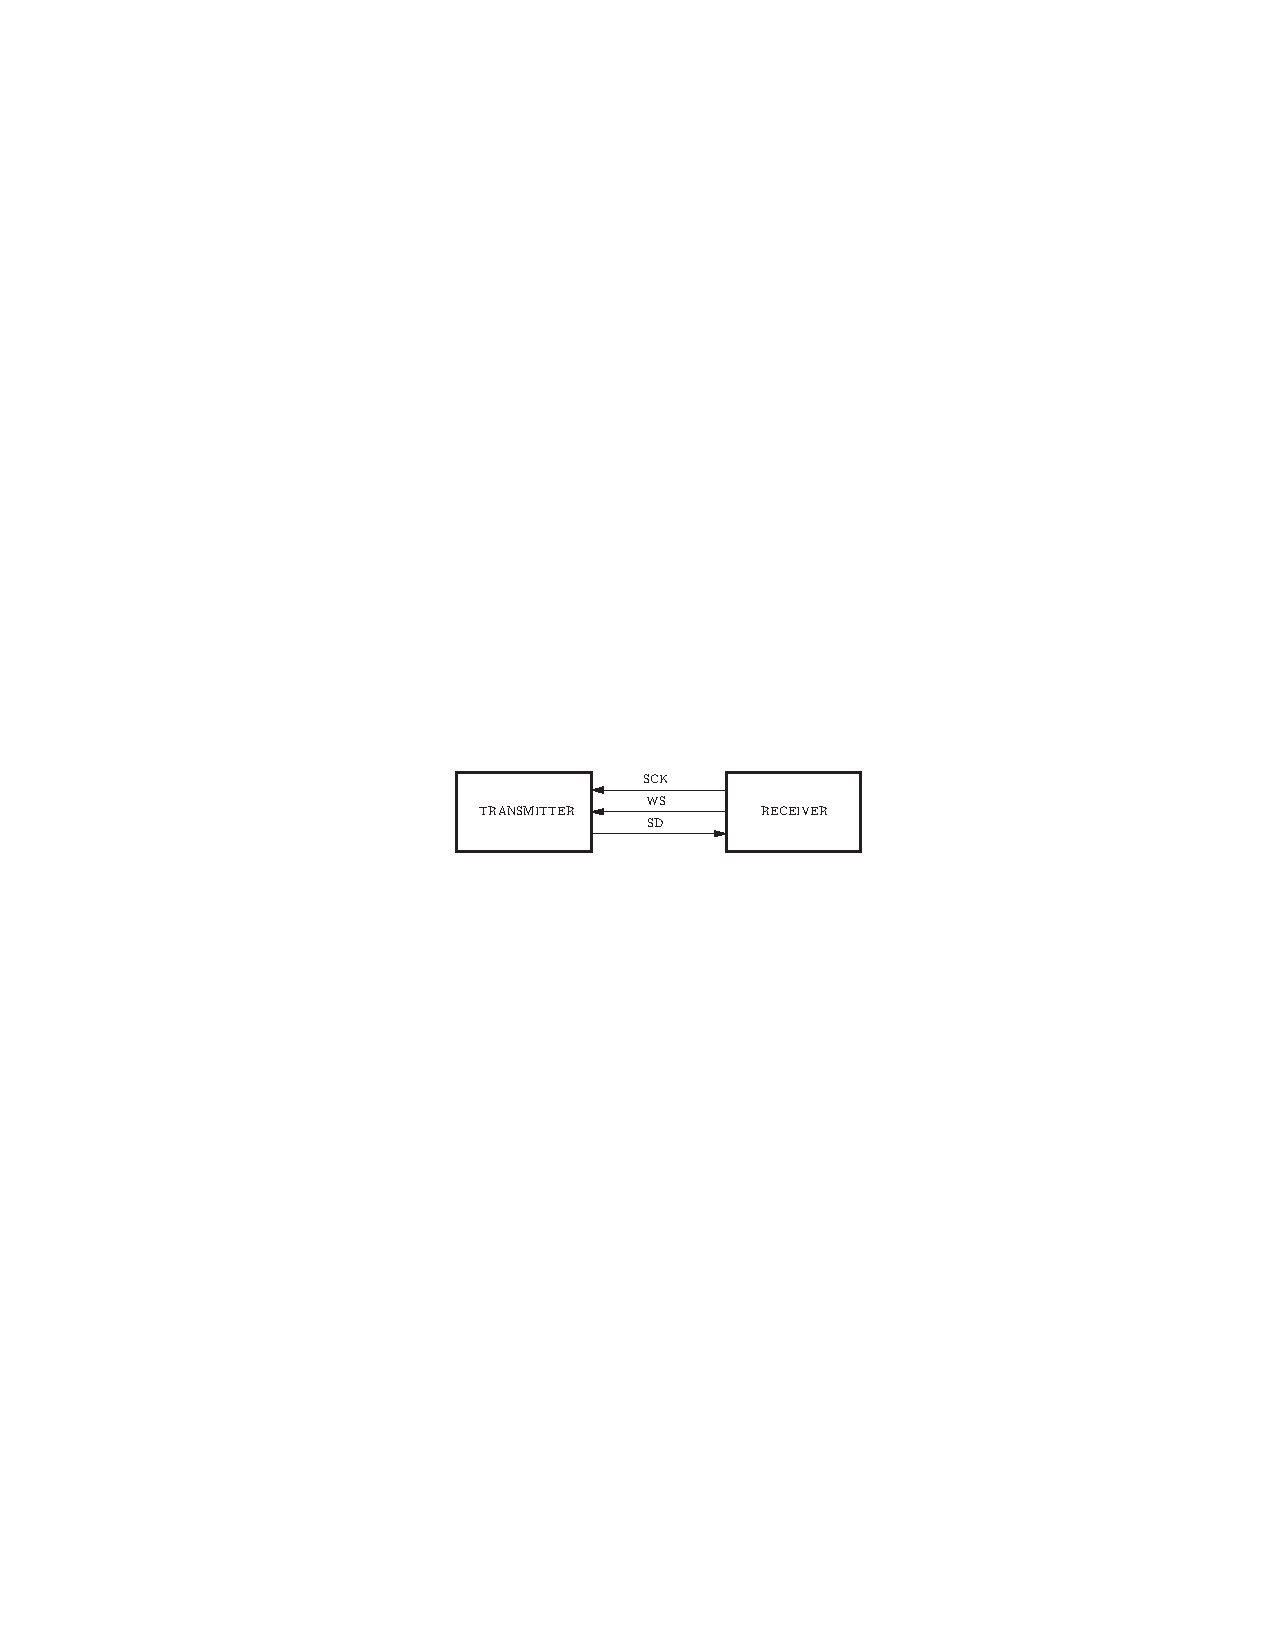
\includegraphics[width=\textwidth]{Hardware/ConfigI2S.pdf}
		\caption{The I2S configuration between the two boards. where Receiver = Master.}
		\label{fig:I2Sconfig}
	\end{subfigure}
	\hfill
	\begin{subfigure}[b]{.45\textwidth}
		\centering
		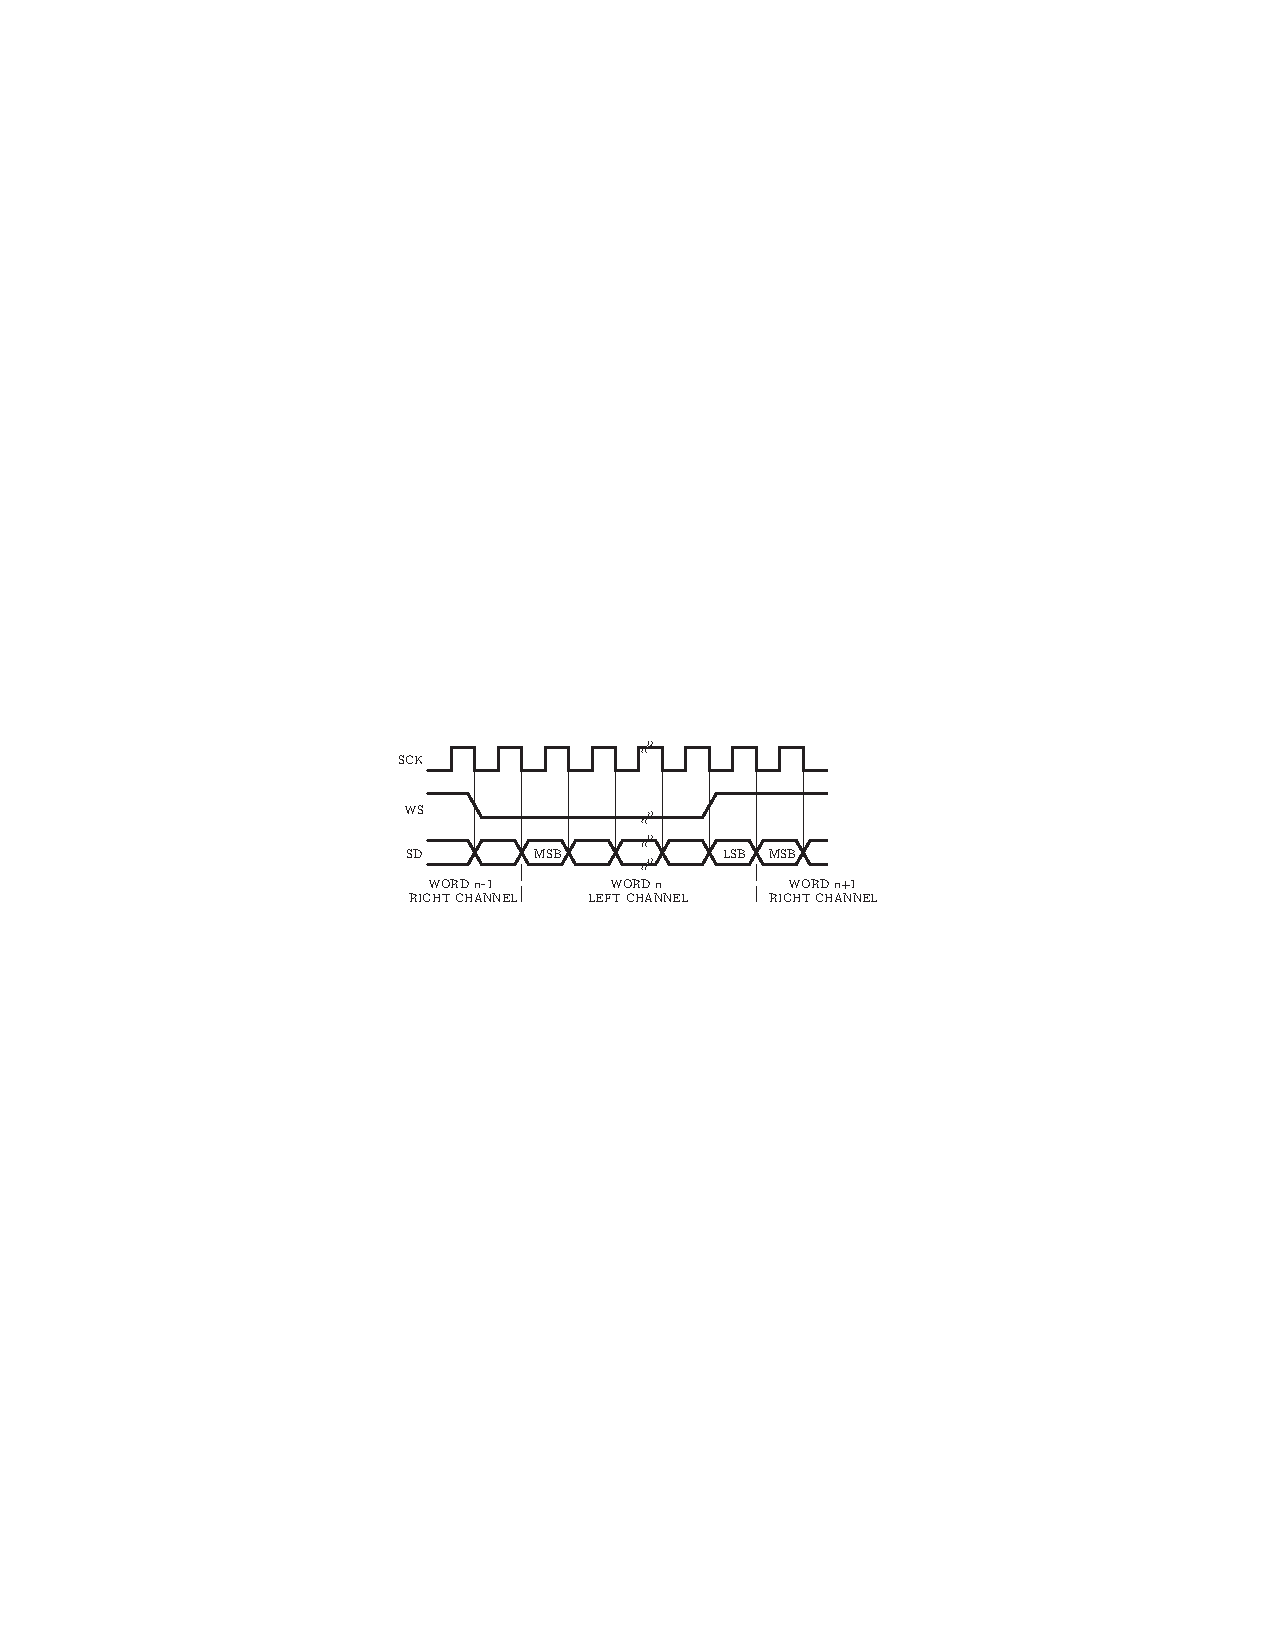
\includegraphics[width=\textwidth]{Hardware/TimingI2S.pdf}
		\caption{The I2S timing interface protocol}
		\label{fig:I2STiming}
	\end{subfigure}	
	\caption{The basic configuration and timing of the I2S protocol.}
\end{figure}

The I2S bus is using regular TTL levels, this is assumed to be handled internally by the boards. The expansion board has been designed to route the master DSP's I2S0 bus together with the slaves I2S2 bus. This has been done purely based on convenience since the TLV320AIC3204 codec is hardwired to the I2S2 bus, making the master DSP's sampling on both buses easier.

\subsubsection*{TLV320AIC3204}

The TLV320AIC3204 codec samples an analogue input with a resolution of 16-bit at a rate of 48 $k$Hz. The gain in both the DAC and ADC can be controlled individually via register 83+84 for the ADC and 65+63 for the DAC. In order to ensure low chance of overflow the gain is tuned to achieve approximately 0x7f00 when max amplitude is reached. The codec is furthermore tuned to have a 0 dB gain of both the ADC and DAC to ensure coherency of the input/output signal.

%The gain is by experiment determined to be:
%\begin{itemize}
%	\item DAC: XX
%	\item ADC: XX
%\end{itemize}
%
%\begin{figure}[H]
%	\centering
%	\begin{subfigure}[b]{.45\textwidth}
%		\centering
%		\includegraphics[width=0.75\textwidth]{missingfigure}
%		\caption{Oscilloscope reading of the input output signal}
%		\label{fig:I2Sconfig}
%	\end{subfigure}
%	\hfill
%	\begin{subfigure}[b]{.45\textwidth}
%		\centering
%		\includegraphics[width=0.75\textwidth]{missingfigure}
%		\caption{Digital readout of the DSP internal memory of the sampled signal}
%		\label{fig:I2STiming}
%	\end{subfigure}	
%	\caption{The figures show the readout from the test used to determine the gain values.}
%\end{figure}


%\subsubsection*{MEMS}
%
%\todo[inline]{not totally sure how this works yet. It's a work in progress}
%
%As mentioned before the TLV320AIC3204 codec have to much delay when sampling the signal, hence the real-time implementation will be depending on MEMS (Micro Electrical Mechanical System) microphones for sampling of ambient sound. These microphones will out their value in a 12-bit value, directly to an I2S port. This will eliminate the AD conversion time and give more time for processing.
%
%The MEMS microphone will only need a serial clock and a data lane from the I2S port.
%
%To be continued..